% !TeX root = ../../book.tex
\hintsection{\Cref*{chGettingStarted}}

在我们开始证明事物之前，我们需要消除某些我们可能试图证明的陈述。考虑下面这句话：

\begin{center} \textit{这句话是假的。} \end{center}
这句话是真的还是假的？如果你仔细思考一下，你就会陷入困境。

再看下面这句话:
\begin{center} \textit{世界上最快乐的驴。} \end{center}
这句话是真的还是假的？好吧，它甚至都不是一个句子；连\textit{问}是真是假的意义都没有！

很明显尝试给出上面了两个陈述的证明是在浪费时间---我们需要将范围缩小到我们实际上可能有机会证明（或可能反驳）的陈述上！这激发了以下（非正式）定义。

\begin{definition}
\label{defProposition}
\label{defProof}
\index{proposition}
\index{proof}
\textbf{命题} \index{proposition}是可以赋予\textbf{真值} (`真' 或 `假')的陈述。如果一个命题为真，则该命题的\textbf{证明}是一个逻辑上有效的论证，证明它是真的，且要达到目标受众可以验证其正确性的水平。
\end{definition}

因此，上面给出的陈述都不是命题，因为没有方法给它们赋予真值。请注意，在 \Cref{defProposition} 中，关键的是说它是真还是假的\textit{合理性}，而不管实际上\textit{是}真还是假---许多命题的真值是未知的，甚至是一些非常简单的命题。

\begin{exercise}
想一个真命题的例子，一个假命题的例子，一个你不知道其真值的命题，以及一个不是命题的陈述。
\end{exercise}

数学论文和教科书中的结论可能被称为\textit{命题}，但根据它们的预期用途，也可能被称为\textit{定理}、\textit{引理}或\textit{推论}。

\begin{itemize} 
\item \textbf{命题} 是一个涵盖性术语，可用于任何结果。
\item \textbf{定理} 是一个特别重要的关键结果。
\item \textbf{引理} 是为了在定理证明中使用而被证明的结果。
\item \textbf{推论} 是无需太多额外工作即可从定理得出的结果。
\end{itemize}

这些不是精确定义，也不是有意而为之---如果你愿意，你可以将每个结果称为一个\textit{命题}---但适当地使用这些词汇可以帮助读者搞清楚如何阅读论文。例如，如果你只想浏览一篇论文并找到其关键结果，您会寻找标记为\textit{定理}的结果。

如果我们没有任何东西可以证明结果，那么试图证明结果就毫无意义。考虑到这一点，我们现在将介绍\textit{数集}，并在整数除法、基数、有理数和无理数、多项式这四个主题的基础上证明关于它们的一些结论，这些主题将为 \Cref{ptCoreConcepts} 中的材料提供背景，并作为对 \Cref{ptTopics} 所涵盖主题的导论。

本章我们不会深入探讨。相反，更像是热身练习---快速、轻松的介绍，并在本书的其余部分提供更多证明。

\subsection*{数集}

在本章后面，以及 \Cref{chSets} 中的详细介绍，我们将遇到\textit{集合}的概念；集合可以被认为是对象的汇集。这个看似简单的概念是数学的基础，它是如此之复杂以至于我们不会在本书中正式地讨论集合。目前，以下定义就足够了。

\begin{definition}[\Cref{defSet}中会被修订]
\label{defSetsPreliminary}
\lindexmmc{in}{$\in$}
\textbf{集合}是对象的汇集。集合中的对象称为集合的\textbf{元素}。如果 $X$ 是一个集合，$x$ 是一个对象，那么 $x \in X$ \inlatexnb{x \textbackslash{}in X} 表示 $x$ 是 $X$ 的一个元素。
\end{definition}

我们首先关注的集合是\textit{数集}---即元素为特定类型的\textit{数}的集合。在入门阶段，许多细节将被暂时掩盖；我们将以适合我们当前阶段的精确程度来讲解，但不妨碍我们发展合理的直觉。

为了定义数集，我们需要三样东西：一条无限长的线、这条线上的一个固定点和一个固定的单位长度。

那我们开始吧。 这是一条无限长的线：
\begin{center}
\begin{tikzpicture}
\draw[latex-latex] (-5.5, 0) -- (5.5, 0) ;
\end{tikzpicture}
\end{center}
箭头表示它应该在两个方向上无限延伸。线上的点代表数字（具体来说，是\textit{实数\textit}，这是一个具有误导性的术语，将在 \Cref{defRealsInformal} 中定义）。现在让我们在这条线上固定一个点，并将其标记为“$0$”：
\begin{center}
\begin{tikzpicture}
\draw[latex-latex] (-5.5, 0) -- (5.5, 0) ; 
\draw (0, 0) -- (0, 0.1) node[above] {$0$} ;
\end{tikzpicture}
\end{center}
这个点可以被认为代表数字零；这是衡量所有其他数字的点。最后，让我们固定一个单位长度：
\begin{center}
\begin{tikzpicture}
\draw (0, 0) -- (1, 0) ; 
\foreach \x in {0,1} \draw (\x, -0.1) -- (\x, 0.1)  ;
\end{tikzpicture}
\end{center}
这个单位长度用于比较其他数字与零的不同程度。

\begin{definition}
\label{defNumberLine}
上述无限直线连同其固定的零点和固定的单位长度，构成了(\textbf{实})\textbf{数轴}。
\end{definition}

我们将用数轴来构造我们感兴趣的五个数字集合：
\begin{itemize}
\item \textit{自然数}集 $\mathbb{N}$ --- \Cref{defNaturalNumbersInformal};
\item \textit{整数}集 $\mathbb{Z}$ --- \Cref{defIntegersInformal};
\item \textit{有理数}集 $\mathbb{Q}$ --- \Cref{defRationalsInformal};
\item \textit{实数}集 $\mathbb{R}$ --- \Cref{defRealsInformal};
\item \textit{复数}集 $\mathbb{C}$ --- \Cref{defComplexNumbersInformal}。
\end{itemize}

正如我们将在本章后面以及整本书中看到的那样，这些集合彼此有着不同的特征，用于不同的目的。

\subsection*{自然数 ($\mathbb{N}$)}

自然数是用于计数的数字---它们是`有多少'类型问题的答案---例如，我有\textit{三}个叔叔、\textit{一}只狗和\textit{零}只猫。

数数是人类长期以来的一项技能。 我们之所以知道这一点，是因为有证据表明人们在数万年前就使用了计数标记。计数标记提供了一种计数较小数字的方法：从零开始，逐一计数你要数的对象，然后为每个对象做一个标记。当完成时，有多少对象就有多少标记。我们从小就被教导用手指数数；这是另一个使用计数标记的例子，只不过我们把做记号变为了伸手指。

做一个计数标记代表数量上的\textit{增加}---即增加一个。在数轴上，我们可以通过向右移动单位长度来表示数量的增加。那么我们从零开始移动的距离，等于我们向右移动单位长度的次数，因此等于被计数对象的数量。

\begin{definition}
\label{defNaturalNumbersInformal}
\textbf{自然数}由数轴上的点表示，可以通过从 $0$ 开始向右移动单位长度任意次获得：
\begin{center}
\begin{tikzpicture}
\draw[latex-latex] (-5.5, 0) -- (5.5, 0) ; 
\foreach \x in {0,1,2,3,4,5} \draw (\x, 0) -- (\x, 0.1) node[above] {$\x$} ;
\end{tikzpicture}
\end{center}
用更熟悉的术语来说，自然数是\textit{非负整数}。全体自然数的集合记作 $\mathbb{N}$ \inlatex{mathbb\{N\}}\lindexmmc{mathbb}{$\mathbb{A}, \mathbb{B}, \dots$}；因此，符号 `$n \in \mathbb{N}$' 表示 $n$ 是一个自然数。
\end{definition}

自然数具有非常重要和有趣的数学结构，并且是 \Cref{chCombinatorics} 中材料的核心。\Cref{secPeanosAxioms} 中将提供对自然数的更加精确的描述，并且可以在 \Cref{secZFC} 中找到自然数集的数学构造（参见 \Cref{cnsNaturalNumbersVonNeumann}）。这些更加精确的描述的核心是`零'和`加一'概念---就像计数标记一样。

\begin{aside}
一些作者将自然数定义为\textit{正}整数，不包括零。我们将 $0$ 视为一个自然数，是因为我们对自然数的主要用途是计算有限集，而一个什么都没有的集合肯定是有限集！也就是说，与任何其他数学定义一样，选择 $0 \in \mathbb{N}$ 还是 $0 \not \in \mathbb{N}$ 只是品味或方便的问题，并且仅仅是一个约定---这不是可以证明或证伪的事情。
\end{aside}

\subsection*{基数}

写下数字现在对你来说似乎轻而易举，但在你小时候可能需要几年时间才能真正理解发生了什么。从历史上看，有许多不同的系统用于象征性地表示数字，即所谓的\textit{数字系统}。\index{numeral system}首先出现的是最原始的计数标记，它出现在石器时代，至今仍被用于某些目的。几千年和数百个数字系统之后，出现了一个占主导地位的数字系统，全世界都知道：\textbf{印度-阿拉伯数字系统}。\index{numeral system!Hindu--Arabic}这个数字系统由十个符号组成，称为\textit{数字}。它是一个\textit{位置}数字系统，意味着符号在字符串中的位置决定了它的数值。

在英语中，这十个数字用\textit{阿拉伯数字}表示：
\[ 0 \quad 1 \quad 2 \quad 3 \quad 4 \quad 5 \quad 6 \quad 7 \quad 8 \quad 9 \]
字符串中最右边的数字在单位位置，每个数字向左移动一位它的数值增加十倍。例如，当我们写下`$2812$'时，最左边的`$2$'代表数字两千，而最后一个`$2$'代表数字二。

事实上，有十个数字，且数字系统基于十的幂，是个生物学巧合，这与大多数人有十根手指这一事实有关。对于许多用途，这是不方便的。 例如， 10 的正因数不多（只有 4 个）---这对执行算术的简易性有影响；基于十二的系统有六个正因数，可能更方便。另一个例子是在计算机和数字电子中，用\textit{二进制}系统会更方便。二进制系统只有2个数字, 分别代表 `关' 和 `开'（或`低电压'和`高电压'）；这样就可以使用电路中的 \textit{逻辑门}序列直接执行算术运算。

因此，了解一些非十进制的位置数字系统是值得的。我们所做的数学抽象带来了 \textit{基数-$b$ 展开} 的定义。

\begin{definition}
\label{defBaseBExpansionPreliminary}
\index{base-$b$ expansion}
\index{number base}
设 $b>1$。自然数 $n$ 的 \textbf{基数-$b$ 展开} 是一个\footnote{这里使用`一个'这个词会引来麻烦，因为它假定每个自然数只有一个基数-$b$ 展开。这个事实实际上需要证明---参见 \Cref{thmBaseBExpansion}。} 字符串 $d_r d_{r-1} \dots d_0$ 满足
\begin{itemize}
\item $n = d_r \cdot b^r + d_{r-1} \cdot b^{r-1} + \cdots + d_0 \cdot b^0$;
\item 对于任意 $i$, $0 \le d_i < b$ for each $i$;
\item 如果 $n>0$ 那么 $d_r \ne 0$---零的基数-$b$ 展开在所有基数 $b$ 上都是 $0$。
\end{itemize}
某些基数有名称；例如，以 $2$ 、 $3$ 、$8$ 、$10$ 和 $16$ 为基数的展开式分别称为\textit{二进制}、\textit{三进制}、\textit{八进制}、\textit{十进制}和\textit{十六进制}。
\end{definition}

\begin{example}
考虑数字 $1023$。他的十进制（基数-$10$）展开为 $1023$，因为
\[ 1023 = 1 \cdot 10^3 + 0 \cdot 10^2 + 2 \cdot 10^1 + 3 \cdot 10^0 \]
它的二进制（基数-$2$）展开为 $1111111111$，因为
\[ 1023 = 1 \cdot 2^9 + 1 \cdot 2^8 + 1 \cdot 2^7 + 1 \cdot 2^6 + 1 \cdot 2^5 + 1 \cdot 2^4 + 1 \cdot 2^3 + 1 \cdot 2^2 + 1 \cdot 2^1 + 1 \cdot 2^0 \]
我们可以用常用的十位数字 $0$ 到 $9$ 和二十六个字母 $\mathrm{A}$ 到 $\mathrm{A}$ 来表示 $36$ 进制的数字；例如，$\mathrm{A}$ 表示 $10$、$\mathrm{M}$ 表示 $22$、$\mathrm{Z}$ 表示 $35$。$1023$ 的基数-$36$ 扩展是 $\mathrm{SF}$，因为

\[ 1023 = 28 \cdot 36^1 + 15 \cdot 36^0 = \mathrm{S} \cdot 36^1 + \mathrm{F} \cdot 36^0 \]
\end{example}

\begin{exercise}
查找数字 $21127$ 的二进制、三进制、八进制、十进制、十六进制和 $36$ 进制的展开，使用字母 $\mathrm{A}$--$\mathrm{F}$ 作为十六进制展开的附加数字，使用字母 $\mathrm{A}$--$\mathrm{Z}$ 作为 $36$ 进制展开的附加数字。
\end{exercise}

我们有时希望用一个自然数的基基数-$b$ 展开来表示它；对此有一些注释。

\begin{notation}
设 $b>1$。如果数字 $d_0,d_1,\dots,d_r$ 是以 $b$ 为基数的数字（在\Creaf{defBaseBExpansionPreliminary}的意义上），那么我们用
\[ {d_rd_{r-1} \dots d_0}_{(b)} = d_r \cdot b^r + d_{r-1} \cdot b^{r-1} + \cdots + d_0 \cdot b^0 \]
表示基数-$b$ 展开为 $d_rd_{r-1} \dots d_0$ 的自然数。如果没有下标 $(b)$ 且没有明确指定基数，则假定展开以 $10$ 为基数。
\end{notation}

\begin{example}
使用新记法，我们有
\[ 1023 = 1111111111_{(2)} = 1101220_{(3)} = 1777_{(8)} = 1023_{(10)} = 3\mathrm{FF}_{(16)} = \mathrm{SF}_{(36)} \]
\end{example}

\subsection*{整数 ($\mathbb{Z}$)}

The \textit{integers} can be used for measuring the difference between two instances of counting. For example, suppose I have five apples and five bananas. Another person, also holding apples and bananas, wishes to trade. After our exchange, I have seven apples and only one banana. Thus I have two more apples and four fewer bananas.

Since an increment in quantity can be represented by moving to the right on the number line by the unit length, a \textit{decrement} in quantity can therefore be represented by moving to the \textit{left} by the unit length. Doing so gives rise to the integers.

\begin{definition}
\label{defIntegersInformal}
The \textbf{integers} are represented by the points on the number line which can be obtained by starting at $0$ and moving in either direction by the unit length any number of times:
\begin{center}
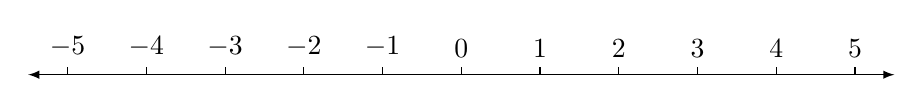
\begin{tikzpicture}
\draw[latex-latex] (-5.5, 0) -- (5.5, 0) ; 
\foreach \x in {-5,-4,-3,-2,-1,0,1,2,3,4,5} \draw (\x, 0) -- (\x, 0.1) node[above] {$\x$} ;
\end{tikzpicture}
\end{center}
We write $\mathbb{Z}$ \inlatex{mathbb\{Z\}}\lindexmmc{mathbb}{$\mathbb{A}, \mathbb{B}, \dots$} for the set of all integers; thus, the notation `$n \in \mathbb{Z}$' means that $n$ is an integer.
\end{definition}

The integers have such a fascinating structure that a whole chapter of this book is devoted to them---see \Cref{chNumberTheory}. This is to do with the fact that, although you can add, subtract and multiply two integers and obtain another integer, the same is not true of division. This `bad behaviour' of division is what makes the integers interesting. We will now see some basic results about division.

\subsection*{整数除法}
\label{pGettingStartedDivision}

The motivation we will soon give for the definition of the rational numbers (\Cref{defRationalsInformal}) is that the result of dividing one integer by another integer is not necessarily another integer. However, the result is \textit{sometimes} another integer; for example, I can divide six apples between three people, and each person will receive an integral number of apples. This makes division interesting: how can we measure the failure of one integer's divisibility by another? How can we deduce when one integer is divisible by another? What is the structure of the set of integers when viewed through the lens of division? This motivates \Cref{defDivisionPreliminary}.

\begin{definition}[to be repeated in \Cref{defDivision}]
\label{defDivisionPreliminary}
\index{division}
\index{divisor}
\index{factor}
\index{multiple}
Let $a,b \in \mathbb{Z}$. We say $b$ \textbf{divides} $a$ if $a=qb$ for some integer $q$. Other ways of saying that $b$ divides $a$ are: $b$ is a \textit{divisor} of $a$, $b$ is a \textit{factor} of $a$, or $a$ is a \textit{multiple} of $b$.
\end{definition}

\begin{example}
The integer $12$ is divisible by $1$, $2$, $3$, $4$, $6$ and $12$, since
\[ 12 = 12 \cdot 1 = 6 \cdot 2 = 4 \cdot 3 = 3 \cdot 4 = 2 \cdot 6 = 1 \cdot 12 \]
It is also divisible by the negatives of all of those numbers; for example, $12$ is divisible by $-3$ since $12 = (-4) \cdot (-3)$.
\end{example}

\begin{exercise}
Prove that $1$ divides every integer, and that every integer divides $0$.
\end{exercise}

Using \Cref{defDivisionPreliminary}, we can prove some general basic facts about divisibility.

\begin{proposition}
\label{propDivisibilityIsTransitive}
Let $a,b,c \in \mathbb{Z}$. If $c$ divides $b$ and $b$ divides $a$, then $c$ divides $a$.
\end{proposition}

\begin{cproof}
Suppose that $c$ divides $b$ and $b$ divides $a$. By \Cref{defDivisionPreliminary}, it follows that
\[ b=qc \quad \text{and} \quad a=rb \]
for some integers $q$ and $r$. Using the first equation, we may substitute $qc$ for $b$ in the second equation, to obtain
\[ a=r(qc) \]
But $r(qc) = (rq)c$, and $rq$ is an integer, so it follows from \Cref{defDivisionPreliminary} that $c$ divides $a$.
\end{cproof}

% To do: draw attention to the wording of the proof, and the 'unpack definition - do something - apply definition' style of the proof.

\begin{exercise}
\label{exDivisibilityIsLinear}
Let $a,b,d \in \mathbb{Z}$. Suppose that $d$ divides $a$ and $d$ divides $b$. Given integers $u$ and $v$, prove that $d$ divides $au+bv$.
\end{exercise}

Some familiar concepts, such as evenness and oddness, can be characterised in terms of divisibility.

\begin{definition}
\label{defEvenOdd}
\index{even!integer}
\index{odd!integer}
An integer $n$ is \textbf{even} if it is divisible by $2$; otherwise, $n$ is \textbf{odd}.
\end{definition}

It is not just interesting to know when one integer \textit{does} divide another; however, proving that one integer \textit{doesn't} divide another is much harder. Indeed, to prove that an integer $b$ does not divide an integer $a$, we must prove that $a \ne qb$ for \textit{any} integer $q$ at all. We will look at methods for doing this in \Cref{chLogicalStructure}; these methods use the following extremely important result, which will underlie all of \Cref{chNumberTheory}.

\begin{theorem}[Division theorem, to be repeated in \Cref{thmDivisionTheorem}]
\label{thmDivisionPreliminary}
\index{division theorem}
Let $a,b \in \mathbb{Z}$ with $b \ne 0$. There is exactly one way to write
\[ a = qb + r \]
such that $q$ and $r$ are integers, and $0 \le r < b$ (if $b > 0$) or $0 \le r < -b$ (if $b < 0$).
\end{theorem}

The number $q$ in \Cref{thmDivisionPreliminary} is called the \textbf{quotient}\index{quotient} of $a$ when divided by $b$, and the number $r$ is called the \textbf{remainder}\index{remainder}.

\begin{example}
The number $12$ leaves a remainder of $2$ when divided by $5$, since $12 = 2 \cdot 5 + 2$.
\end{example}

Here's a slightly more involved example.

\begin{proposition}
Suppose an integer $a$ leaves a remainder of $r$ when divided by an integer $b$, and that $r>0$. Then $-a$ leaves a remainder of $b-r$ when divided by $b$.
\end{proposition}

\begin{cproof}
Suppose $a$ leaves a remainder of $r$ when divided by $b$. Then
\[ a=qb+r \]
for some integer $q$. A bit of algebra yields
\[ -a = -qb-r = -qb-r+(b-b) = -(q+1)b + (b-r) \]
Since $0<r<b$, we have $0<b-r<b$. Hence $-(q+1)$ is the quotient of $-a$ when divided by $b$, and $b-r$ is the remainder.
\end{cproof}

\begin{exercise}
Prove that if an integer $a$ leaves a remainder of $r$ when divided by an integer $b$, then $a$ leaves a remainder of $r$ when divided by $-b$.
\end{exercise}

We will finish this part on division of integers by connecting it with the material on number bases---we can use the division theorem (\Cref{thmDivisionPreliminary}) to find the base-$b$ expansion of a given natural number. It is based on the following observation: the natural number $n$ whose base-$b$ expansion is $d_rd_{r-1} \cdots d_1 d_0$ is equal to
\[ d_0 + b(d_1 + b(d_2 + \cdots + b(d_{r-1} + bd_r) \cdots)) \]
Moreover, $0 \le d_i < b$ for all $i$. In particular $n$ leaves a remainder of $d_0$ when divided by $b$. Hence
\[ \frac{n-d_0}{b} = d_1 + d_2b + \cdots + d_rb^{r-1} \]
The base-$b$ expansion of $\frac{n-d_0}{b}$ is therefore
\[ d_rd_{r-1} \cdots d_1 \]
In other words, the remainder of $n$ when divided by $b$ is the last base-$b$ digit of $n$, and then subtracting this number from $n$ and dividing the result by $b$ truncates the final digit. Repeating this process gives us $d_1$, and then $d_2$, and so on, until we end up with $0$.

This suggests the following algorithm for computing the base-$b$ expansion of a number $n$:
\begin{itemize}
\item \textbf{Step 1.} Let $d_0$ be the remainder when $n$ is divided by $b$, and let $n_0=\frac{n-d_0}{b}$ be the quotient. Fix $i=0$.
\item \textbf{Step 2.} Suppose $n_i$ and $d_i$ have been defined. If $n_i=0$, then proceed to Step 3. Otherwise, define $d_{i+1}$ to be the remainder when $n_i$ is divided by $b$, and define $n_{i+1} = \frac{n_i-d_{i+1}}{b}$. Increment $i$, and repeat Step 2.
\item \textbf{Step 3.} The base-$b$ expansion of $n$, is
\[ d_id_{i-1} \cdots d_0 \]
\end{itemize}

\begin{example}
We compute the base-$17$ expansion of $15213$, using the letters $\mathrm{A}$--$\mathrm{G}$ to represent the numbers $10$ through $16$.
\begin{itemize}
\item $15213 = 894 \cdot 17 + 15$, so $d_0=15=\mathrm{F}$ and $n_0=894$.
\item $894 = 52 \cdot 17 + 10$, so $d_1=10 = \mathrm{A}$ and $n_1=52$.
\item $52 = 3 \cdot 17 + 1$, so $d_2 = 1$ and $n_2=3$.
\item $3 = 0 \cdot 17 + 3$, so $d_3 = 3$ and $n_3=0$.
\item The base-$17$ expansion of $15213$ is therefore $31\mathrm{AF}$.
\end{itemize}
A quick verification gives
\[ 31\mathrm{AF}_{(17)} = 3 \cdot 17^3 + 1 \cdot 17^2 + 10 \cdot 17 + 15 = 15213 \]
as desired.
\end{example}

\begin{exercise}
Find the base-$17$ expansion of $408\,735\,787$ and the base-$36$ expansion of $1\,442\,151\,747$.
\end{exercise}

\subsection*{有理数 ($\mathbb{Q}$)}

Bored of eating apples and bananas, I buy a pizza which is divided into eight slices. A friend and I decide to share the pizza. I don't have much of an appetite, so I eat three slices and my friend eats five. Unfortunately, we cannot represent the proportion of the pizza each of us has eaten using natural numbers or integers. However, we're not far off: we can count the number of equal parts the pizza was split into, and of those parts, we can count how many we had. On the number line, this could be represented by splitting the unit line segment from $0$ to $1$ into eight equal pieces, and proceeding from there. This kind of procedure gives rise to the \textit{rational numbers}.

\begin{definition}
\label{defRationalsInformal}
The \textbf{rational numbers} are represented by the points at the number line which can be obtained by dividing any of the unit line segments between integers into an equal number of parts.
\begin{center}
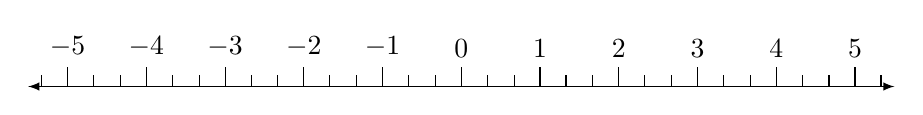
\begin{tikzpicture}
\draw[latex-latex] (-5.5, 0) -- (5.5, 0) ; 
\foreach \x in {-5,-4,-3,-2,-1,0,1,2,3,4,5} \draw (\x, 0) -- (\x, 0.25) node[above] {$\x$} ;
\foreach \x in {-5,-4,-3,-2,-1,0,1,2,3,4,5} {
  \foreach \i in {-0.33,0.33} {
    \draw (\x+\i, 0) -- (\x+\i, 0.15) ;
  }
}
\end{tikzpicture}
\end{center}
The rational numbers are those of the form $\frac{a}{b}$, where $a,b \in \mathbb{Z}$ and $b \ne 0$. We write $\mathbb{Q}$ \inlatex{mathbb\{Q\}}\lindexmmc{mathbb}{$\mathbb{A}, \mathbb{B}, \dots$} for the set of all rational numbers; thus, the notation `$q \in \mathbb{Q}$' means that $q$ is a rational number.
\end{definition}

The rational numbers are a very important example of a type of algebraic structure known as a \textit{field}---they are particularly central to algebraic number theory and algebraic geometry.

\subsection*{实数 ($\mathbb{R}$)}

Quantity and change can be measured in the abstract using \textit{real numbers}.

\begin{definition}
\label{defRealsInformal}
The \textbf{real numbers} are the points on the number line. We write $\mathbb{R}$ \inlatex{mathbb\{R\}}\lindexmmc{mathbb}{$\mathbb{A}, \mathbb{B}, \dots$} for the set of all real numbers; thus, the notation `$a \in \mathbb{R}$' means that $a$ is a real number.
\end{definition}

The real numbers are central to real analysis, a branch of mathematics introduced in \Cref{chRealNumbers}. They turn the rationals into a \textit{continuum} by `filling in the gaps'---specifically, they have the property of \textit{completeness}, meaning that if a quantity can be approximated with arbitrary precision by real numbers, then that quantity is itself a real number.

We can define the basic arithmetic operations (addition, subtraction, multiplication and division) on the real numbers, and a notion of ordering of the real numbers, in terms of the infinite number line.

\begin{itemize}
\item \textbf{Ordering.} A real number $a$ is less than a real number $b$, written $a<b$, if $a$ lies to the left of $b$ on the number line. The usual conventions for the symbols $\le$ \inlatex{le}\lindexmmc{le}{$\le$}, $>$ and $\ge$ \inlatex{ge}\lindexmmc{ge}{$\ge$} apply, for instance `$a \le b$' means that either $a < b$ or $a = b$.

\item \textbf{Addition.} Suppose we want to add a real number $a$ to a real number $b$. To do this, we \textit{translate} $a$ by $b$ units to the right---if $b<0$ then this amounts to translating $a$ by an equivalent number of units to the left. Concretely, take two copies of the number line, one above the other, with the same choice of unit length; move the $0$ of the lower number line beneath the point $a$ of the upper number line. Then $a+b$ is the point on the upper number line lying above the point $b$ of the lower number line.

Here is an illustration of the fact that $(-3) + 5 = 2$:

\begin{center}
\fitwidthc{0.9}{\begin{tikzpicture}
% Adapted from http://tex.stackexchange.com/questions/148252/
\draw[latex-latex] (-8.5,0) -- (5.5,0) ; 
\foreach \x in  {-8,-7,-6,-5,-4,-3,-2,-1,0,1,2,3,4,5}
\draw[shift={(\x,0)}] (0pt,3pt) -- (0pt,-3pt);
\foreach \x in {-8,-7,-6,-5,-4,-3,-2,-1,0,1,2,3,4,5}
\draw[shift={(\x,0)}] (0pt,0pt) -- (0pt,3pt) node[above] {$\x$};
\draw[*-*] (-3.08,0) -- (2.08,0);
\draw[very thick] (-3,0) -- (2,0);

\draw[latex-latex] (-8.5,-1) -- (5.5,-1) ; 
\foreach \x in  {-5,-4,-3,-2,-1,0,1,2,3,4,5,6,7,8}
\draw[shift={(\x-3,-1)},color=black] (0pt,3pt) -- (0pt,-3pt);
\foreach \x in {-5,-4,-3,-2,-1,0,1,2,3,4,5,6,7,8}
\draw[shift={(\x-3,-1)},color=black] (0pt,0pt) -- (0pt,-3pt) node[below] {$\x$};
\draw[dashed] (-3,-1) -- (-3,0) ;
\draw[->] (2,-0.8) -- (2,-0.2) ;
\end{tikzpicture}}
\end{center}

\item \textbf{Multiplication.} This one is fun. Suppose we want to multiply a real number $a$ by a real number $b$. To do this, we \textit{scale} the number line, and perhaps \textit{reflect} it. Concretely, take two copies of the number line, one above the other; align the $0$ points on both number lines, and stretch the lower number line evenly until the point $1$ on the lower number line is below the point $a$ on the upper number line---note that if $a<0$ then the number line must be reflected in order for this to happen. Then $a \cdot b$ is the point on the upper number line lying above $b$ on the lower number line.

Here is an illustration of the fact that $5 \cdot 4 = 20$.

\begin{center}
\fitwidthc{0.9}{\begin{tikzpicture}
% Adapted from http://tex.stackexchange.com/questions/148252/
\draw[latex-latex] (-5.5,0) -- (8.5,0) ; 
\foreach \x in  {-2,-1,0,1,2,3,4,5,6,7,8,9,10,11,12,13,14,15,16,17,18,19,20,21,22,23,24}
\draw[shift={(0.5*\x-4,0)}] (0pt,3pt) -- (0pt,-3pt);
\foreach \x in {-2,-1,0,1,2,3,4,5,6,7,8,9,10,11,12,13,14,15,16,17,18,19,20,21,22,23,24}
\draw[shift={(0.5*\x-4,0)}] (0pt,0pt) -- (0pt,3pt) node[above] {$\text{\footnotesize\x}$};
\draw[*-*] (-1.58,0) -- (6.08,0);
\draw[very thick] (-1.5,0) -- (6,0);

\draw[latex-latex] (-5.5,-1) -- (8.5,-1) ; 
\foreach \x in  {0,1,2,3,4}
\draw[shift={(2.5*\x-4,-1)},color=black] (0pt,3pt) -- (0pt,-3pt);
\foreach \x in {0,1,2,3,4}
\draw[shift={(2.5*\x-4,-1)},color=black] (0pt,0pt) -- (0pt,-3pt) node[below] {$\x$};
\draw[dashed] (-4,-1) -- (-4,0) ;
\draw[dashed] (-1.5,-1) -- (-1.5,0) ;
\draw[->] (6,-0.8) -- (6,-0.2) ;
\end{tikzpicture}}
\end{center}

and here is an illustration of the fact that $(-5) \cdot 4 = -20$:
\begin{center}
\fitwidthc{0.9}{\begin{tikzpicture}
% Adapted from http://tex.stackexchange.com/questions/148252/
\draw[latex-latex] (-5.5,0) -- (8.5,0) ; 
\foreach \x in  {-22,-21,...,4}
\draw[shift={(0.5*\x+6,0)}] (0pt,3pt) -- (0pt,-3pt);
\foreach \x in {-22,-21,...,4}
\draw[shift={(0.5*\x+6,0)}] (0pt,0pt) -- (0pt,3pt) node[above] {$\text{\footnotesize\x}$};
\draw[*-*] (-4.08,0) -- (3.58,0);
\draw[very thick] (-4,0) -- (3.5,0);

\draw[latex-latex] (-5.5,-1) -- (8.5,-1) ; 
\foreach \x in  {0,1,2,3,4}
\draw[shift={(6-2.5*\x,-1)},color=black] (0pt,3pt) -- (0pt,-3pt);
\foreach \x in {0,1,2,3,4}
\draw[shift={(6-2.5*\x,-1)},color=black] (0pt,0pt) -- (0pt,-3pt) node[below] {$\x$};
\draw[dashed] (6,-1) -- (6,0) ;
\draw[dashed] (3.5,-1) -- (3.5,0) ;
\draw[->] (-4,-0.8) -- (-4,-0.2) ;
\end{tikzpicture}}
\end{center}
\end{itemize}

\begin{exercise}
Interpret the operations of subtraction and division as geometric transformations of the real number line.
\end{exercise}

We will take for granted the arithmetic properties of the real numbers in this chapter, waiting until \Cref{secInequalitiesMeans} to sink our teeth into the details. For example, we will take for granted the basic properties of rational numbers, for instance
\[ \frac{a}{b}+\frac{c}{d} = \frac{ad+bc}{bd} \quad \text{and} \quad \frac{a}{b} \cdot \frac{c}{d} = \frac{ac}{bd} \]

\subsection*{有理数和无理数}
\label{pGettingStartedRationalNumbers}

Before we can talk about irrational numbers, we should say what they are.

\begin{definition}
\label{defIrrationalNumber}
\index{irrational number}
An \textbf{irrational number} is a real number that is not rational.
\end{definition}

Unlike $\mathbb{N},\mathbb{Z},\mathbb{Q},\mathbb{R},\mathbb{C}$, there is no standard single letter expressing the irrational numbers. However, by the end of \Cref{secSetOperations}, we will be able to write the set of irrational numbers as $\mathbb{R} \setminus \mathbb{Q}$.

Note in particular that `irrational' does not simply mean `not rational'---that would imply that all complex numbers which are not real are irrational---rather, the term `irrational' means `real and not rational'.

Proving that a real number is \textit{irrational} is not particularly easy. We will get our foot in the door by allowing ourselves to assume the following result, which is restated and proved in \Cref{propSqrt2Irrational}.

\begin{proposition}
\label{propSqrt2IrrationalPreliminary}
The real number $\sqrt{2}$ is irrational. \qed
\end{proposition}

We can use the fact that $\sqrt{2}$ is irrational to prove some facts about the relationship between rational numbers and irrational numbers.

\begin{proposition}
Let $a$ and $b$ be irrational numbers. It is possible that $ab$ be rational.
\end{proposition}

\begin{cproof}
Let $a=b=\sqrt{2}$. Then $a$ and $b$ are irrational, and $ab=2=\frac{2}{1}$, which is rational.
\end{cproof}

\begin{exercise}
Let $r$ be a rational number and let $a$ be an irrational number. Prove that it is possible that $ra$ be rational, and it is possible that $ra$ be irrational.
\end{exercise}

\subsection*{复数 ($\mathbb{C}$)}

We have seen that multiplication by real numbers corresponds with scaling and reflection of the number line---scaling alone when the multiplicand is positive, and scaling with reflection when it is negative. We could alternatively interpret this reflection as a \textit{rotation} by half a turn, since the effect on the number line is the same. You might then wonder what happens if we rotate by arbitrary angles, rather than only half turns.

What we end up with is a \textit{plane} of numbers, not merely a line---see \Cref{figComplexNumbers}. Moreover, it happens that the rules that we expect arithmetic operations to satisfy still hold---addition corresponds with translation, and multiplication corresponds with scaling and rotation. This resulting number set is that of the \textit{complex numbers}.

\begin{definition}
\label{defComplexNumbersInformal}
The \textbf{complex numbers} are those obtained by the non-negative real numbers upon rotation by any angle about the point $0$. We write $\mathbb{C}$ \inlatex{mathbb\{C\}}\lindexmmc{mathbb}{$\mathbb{A}, \mathbb{B}, \dots$} for the set of all complex numbers; thus, the notation `$z \in \mathbb{C}$' means that $z$ is a complex number.
\end{definition}

\begin{figure}[p!]
\centering
\resizebox{\textwidth}{!}{
\begin{tikzpicture}
\draw[latex-latex] (-5.5,0) -- (5.5,0) ;
\draw[latex-latex, dotted] (-4.76, 2.75) -- (4.76, -2.75) ;
\draw[latex-latex, dotted] (-2.75, 4.76) -- (2.75, -4.76) ;
\draw[latex-latex, dotted] (0, -5.5) -- (0, 5.5) ;
\draw[latex-latex, dotted] (2.75, 4.76) -- (-2.75, -4.76) ;
\draw[latex-latex, dotted] (4.76, 2.75) -- (-4.76, -2.75) ;
\draw[dotted] (0,0) circle [radius=1] ;
\draw[dotted] (0,0) circle [radius=2] ;
\draw[dotted] (0,0) circle [radius=3] ;
\draw[dotted] (0,0) circle [radius=4] ;
\draw[dotted] (0,0) circle [radius=5] ;
\foreach \x in  {-5,-4,-3,-2,-1,0,1,2,3,4,5}
  \draw[shift={(\x,0)}] (0pt,3pt) -- (0pt,-3pt);
\foreach \x in {-5,-4,-3,-2,-1,0,1,2,3,4,5}
  \draw[shift={(\x,0)}] (0,0) node[below right] {$\text{\small\x}$};
\draw (0,1) node[above right] {$i$};
\draw (-3pt,1) -- (3pt,1);
\foreach \x in {2,3,4,5}
  \draw[shift={(0,\x)}] (0,0) node[above right] {$\x i$};
\foreach \x in {2,3,4,5}
  \draw[shift={(0,\x)}] (-3pt,0pt) -- (3pt, 0pt);
\foreach \x in {2,3,4,5}
  \draw[shift={(0,-\x)}] (0,0) node[below right] {$\text{\small-}\x i$};
\foreach \x in {2,3,4,5}
  \draw[shift={(0,-\x)}] (-3pt,0pt) -- (3pt, 0pt);
\draw (0,-1) node[below right] {$\text{\small-}i$};
\draw (-3pt,-1) -- (3pt,-1);
\end{tikzpicture}
}
\caption{Illustration of the complex plane, with some points labelled.}
\label{figComplexNumbers}
\end{figure}

There is a particularly important complex number, $i$, which is the point in the complex plane exactly one unit above $0$---this is illustrated in \Cref{figComplexNumbers}. Multiplication by $i$ has the effect of rotating the plane by a quarter turn anticlockwise. In particular, we have $i^2 = i \cdot i = -1$; the complex numbers have the astonishing property that square roots of \textit{all} complex numbers exist (including all the real numbers).

In fact, every complex number can be written in the form $a+bi$, where $a,b \in \mathbb{R}$; this number corresponds with the point on the complex plane obtained by moving $a$ units to the right and $b$ units up, reversing directions as usual if $a$ or $b$ is negative. Arithmetic on the complex numbers works just as with the real numbers; in particular, using the fact that $i^2=-1$, we obtain
\[ (a+bi)+(c+di) = (a+c)+(b+d)i \quad \text{and} \quad (a+bi) \cdot (c+di) = (ac-bd) + (ad+bc)i \]

We will discuss complex numbers further in the portion of this chapter on polynomials below.

\subsection*{多项式}
\label{pGettingStartedPolynomials}

The natural numbers, integers, rational numbers, real numbers and complex numbers are all examples of \textit{semirings}, which means that they come equipped with nicely behaving notions of addition and multiplication.

\begin{definition}
\label{defPolynomialPreliminary}
\index{polynomial}
Let $\mathbb{S} = \mathbb{N}$, $\mathbb{Z}$, $\mathbb{Q}$, $\mathbb{R}$ or $\mathbb{C}$. A (\textbf{univariate}) \textbf{polynomial over $\mathbb{S}$} in the \textbf{indeterminate} $x$ is an expression of the form
\[ a_0 + a_1x + \cdots + a_nx^n \]
where $n \in \mathbb{N}$ and each $a_k \in \mathbb{S}$. The numbers $a_k$ are called the \textbf{coefficients} of the polynomial. If not all coefficients are zero, the largest value of $k$ for which $a_k \ne 0$ is called the \textbf{degree} of the polynomial. By convention, the degree of the polynomial $0$ is $-\infty$.
\end{definition}

Polynomials of degree $1$, $2$, $3$, $4$ and $5$ are respectively called \textit{linear}, \textit{quadratic}, \textit{cubic}, \textit{quartic} and \textit{quintic} polynomials.

\begin{example}
The following expressions are all polynomials:
\[ 3 \qquad 2x-1 \qquad (3+i)x^2-x \]
Their degrees are $0$, $1$ and $2$, respectively. The first two are polynomials over $\mathbb{Z}$, and the third is a polynomial over $\mathbb{C}$.
\end{example}

\begin{exercise}
Write down a polynomial of degree $4$ over $\mathbb{R}$ which is not a polynomial over $\mathbb{Q}$.
\end{exercise}

\begin{notation}
Instead of writing out the coefficients of a polynomial each time, we may write something like $p(x)$ or $q(x)$. The `$(x)$' indicates that $x$ is the indeterminate of the polynomial. If $\alpha$ is a number\footnote{When dealing with polynomials, we will typically reserve the letter $x$ for the indeterminate variable, and use the Greek letters $\alpha,\beta,\gamma$ \inlatex{alpha, \textbackslash{}beta, \textbackslash{}gamma} for numbers to be substituted into a polynomial.} and $p(x)$ is a polynomial in indeterminate $x$, we write $p(\alpha)$ for the result of \textbf{substituting} $\alpha$ for $x$ in the expression $p(x)$.
\end{notation}

Note that, if $A$ is any of the sets $\mathbb{N}$, $\mathbb{Z}$, $\mathbb{Q}$, $\mathbb{R}$ or $\mathbb{C}$, and $p(x)$ is a polynomial over $A$, then $p(\alpha) \in A$ for all $\alpha \in A$.

\begin{example}
Let $p(x)=x^3-3x^2+3x-1$. Then $p(x)$ is a polynomial over $\mathbb{Z}$ with indeterminate $x$. For any integer $\alpha$, the value $p(\alpha)$ will also be an integer. For example
\[ p(0) = 0^3-3 \cdot 0^2 + 3 \cdot 0 - 1 = -1 \quad \text{and} \quad p(3) = 3^3 - 3 \cdot 3^2 + 3 \cdot 3 - 1 = 8 \]
\end{example}

\begin{definition}
\label{defRootOfPolynomial}
\index{root}
Let $p(x)$ be a polynomial. A \textbf{root} of $p(x)$ is a complex number $\alpha$ such that $p(\alpha)=0$.
\end{definition}

The \textit{quadratic formula} (\Cref{thmQuadraticFormula}) tells us that the roots of the polynomial $x^2+ax+b$, where $a,b \in \mathbb{C}$, are precisely the complex numbers
\[ \frac{-a+\sqrt{a^2-4b}}{2} \quad \text{and} \quad \frac{-a-\sqrt{a^2-4b}}{2} \]

Note our avoidance of the symbol `$\pm$', which is commonly found in discussions of quadratic polynomials. The symbol `$\pm$' is dangerous because it may suppress the word `and' or the word `or', depending on context---this kind of ambiguity is not something that we will want to deal with when discussing the logical structure of a proposition in \Cref{chLogicalStructure}!

\begin{example}
\label{exApplicationOfQuadraticFormula}
Let $p(x)=x^2-2x+5$. The quadratic formula tells us that the roots of $p$ are
\begin{center}
$\dfrac{2 + \sqrt{4 - 4 \cdot 5}}{2} = 1 + \sqrt{-4} = 1+2i$
\quad and \quad
$\dfrac{2 - \sqrt{4 - 4 \cdot 5}}{2} = 1-\sqrt{-4} = 1-2i$
\end{center}
The numbers $1+2i$ and $1-2i$ are related in that their real parts are equal and their imaginary parts differ only by a sign. \Cref{exComplexNumberAsRootOfQuadraticOverR} generalises this observation.
\end{example}

\begin{exercise}
\label{exComplexNumberAsRootOfQuadraticOverR}
Let $\alpha = a+bi$ be a complex number, where $a,b \in \mathbb{R}$. Prove that $\alpha$ is the root of a quadratic polynomial over $\mathbb{R}$, and find the other root of this polynomial.
\end{exercise}

The following exercise proves the well-known result which classifies the number of real roots of a polynomial over $\mathbb{R}$ in terms of its coefficients.

\begin{exercise}
\label{exDiscriminantRealRoots}
\index{discriminant}
Let $a,b \in \mathbb{C}$ and let $p(x)=x^2+ax+b$. The value $\Delta=a^2-4b$ is called the \textbf{discriminant} of $p$. Prove that $p$ has two roots if $\Delta \ne 0$ and one root if $\Delta = 0$. Moreover, if $a,b \in \mathbb{R}$, prove that $p$ has no real roots if $\Delta < 0$, one real root if $\Delta = 0$, and two real roots if $\Delta > 0$.
\end{exercise}

\begin{example}
Consider the polynomial $x^2-2x+5$. Its discriminant is equal to $(-2)^2-4 \cdot 5 = -16$, which is negative. \Cref{exDiscriminantRealRoots} tells us that it has two roots, neither of which are real. This was verified by \Cref{exApplicationOfQuadraticFormula}, where we found that the roots of $x^2-2x+5$ are $1+2i$ and $1-2i$.

Now consider the polynomial $x^2-2x-3$. Its discriminant is equal to $(-2)^2-4\cdot(-3) = 16$, which is positive. \Cref{exDiscriminantRealRoots} tells us that it has two roots, both of which are real; and indeed
\[ x^2-2x-3 = (x+1)(x-3) \]
so the roots of $x^2-2x-3$ are $-1$ and $3$.
\end{example}